\documentclass[runningheads]{llncs}

\usepackage[T1]{fontenc}
\usepackage{url}
\usepackage{graphicx}
\usepackage{float}
\usepackage{listings}
\usepackage{xcolor}
\usepackage{enumitem}
\usepackage{subcaption}

% Configurare pentru code snippets
\lstset{
    basicstyle=\ttfamily\small,
    breaklines=true,
    frame=single,
    language=C++,
    commentstyle=\color{gray},
    keywordstyle=\color{blue},
    stringstyle=\color{red},
    showstringspaces=false
}

\begin{document}

\title{NetworkDevicesMonitor}

\author{Ivaniciuc Teodor-Arsenie}

\institute{Universitatea "Alexandru Ioan Cuza" din Iasi, Facultatea de Informatica \\
Iasi, Romania \\
\email{teodor-arsenie.ivaniciuc@info.uaic.ro} 
}

\maketitle

\begin{abstract}
NetworkDevicesMonitor este o platforma software completa pentru monitorizarea si analiza infrastructurii IT, integrand protocoale standardizate (Syslog) cu agenti personalizati pentru colectarea telemetriei. Arhitectura multi-threaded implementeaza pattern-uri avansate (Producer-Consumer, Thread-Safe Queues) si ofera o interfata grafica asincrona Qt6 cu dashboard-uri interactive, vizualizari în timp real, sistem de alertare automata si filtrare avansata.  Proiectul demonstreaza aplicarea conceptelor de retele, concurenta, baze de date si design UI/UX profesional, incluzand functionalitati complete de securitate prin whitelist/blacklist, management alerte personalizate si filtre dinamice.
\end{abstract}

\section{Introducere si Context}

\subsection{Motivatie}
În infrastructurile IT moderne, echipamentele de retea (routere, switch-uri, firewall-uri) si statiile de lucru genereaza volume masive de date sub forma de log-uri si metrici. Monitorizarea manuala devine rapid impracticabila, conducand la:  
\begin{itemize}[itemsep=0em]
    \item Pierderea evenimentelor critice de securitate
    \item Dificultati în diagnosticarea problemelor de performanta
    \item Lipsa vizibilitatii centralizate asupra infrastructurii
    \item Timp de raspuns crescut la incidente
    \item Absenta filtrarii inteligente a datelor relevante
    \item Management ineficient al alertelor si notificarilor
\end{itemize}

\subsection{Obiective Tehnice}
NetworkDevicesMonitor adreseaza aceste provocari prin:  

\begin{enumerate}
    \item \textbf{Colectare Hibrida: } 
    \begin{itemize}
        \item Syslog (RFC 5424) pe portul 1514 pentru echipamente standard
        \item Agenti custom pe portul 9000 pentru metrici detaliate (CPU, RAM, disk)
        \item Protocol JUNK pe portul 8080 pentru comunicare client-server
    \end{itemize}
    
    \item \textbf{Procesare Concurenta Performanta:}
    \begin{itemize}
        \item I/O Multiplexing cu \texttt{poll()} pentru receptie non-blocanta
        \item Thread-Safe Queues pentru decuplarea ingestiei de procesare
        \item Worker threads pentru parsing si analiza paralela
        \item Shared mutex pentru operatiuni concurrent read-heavy
    \end{itemize}
    
    \item \textbf{Securitate prin Filtrare Multi-Nivel:}
    \begin{itemize}
        \item Source Manager cu Whitelist/Blacklist IP-uri
        \item Validare automata a surselor înainte de procesare
        \item Izolare trafic malitios si unknown sources
        \item Filtre personalizate pe tip, mesaj si alerte custom
    \end{itemize}
    
    \item \textbf{Vizualizare si UX Avansat:}
    \begin{itemize}
        \item Dashboard asincron Qt6 cu actualizari în timp real
        \item Grafice interactive (Donut Charts, Line Charts)
        \item Sistem de alertare pop-up pentru evenimente critice
        \item Pagini dedicate pentru Syslog, Agents, Security si Filtres
    \end{itemize}
    
    \item \textbf{Management Avansat:}
    \begin{itemize}
        \item Sistem de filtrare dinamica (type, message, custom alerts)
        \item Management centralizat al alertelor cu rezolvare
        \item Separare date cunoscute vs.  unknown sources
    \end{itemize}
\end{enumerate}

\section{Arhitectura Sistemului}

\subsection{Vedere de Ansamblu}
Sistemul este structurat în 3 componente majore care comunica prin protocoale TCP:  

\begin{figure}[H]
    \centering
    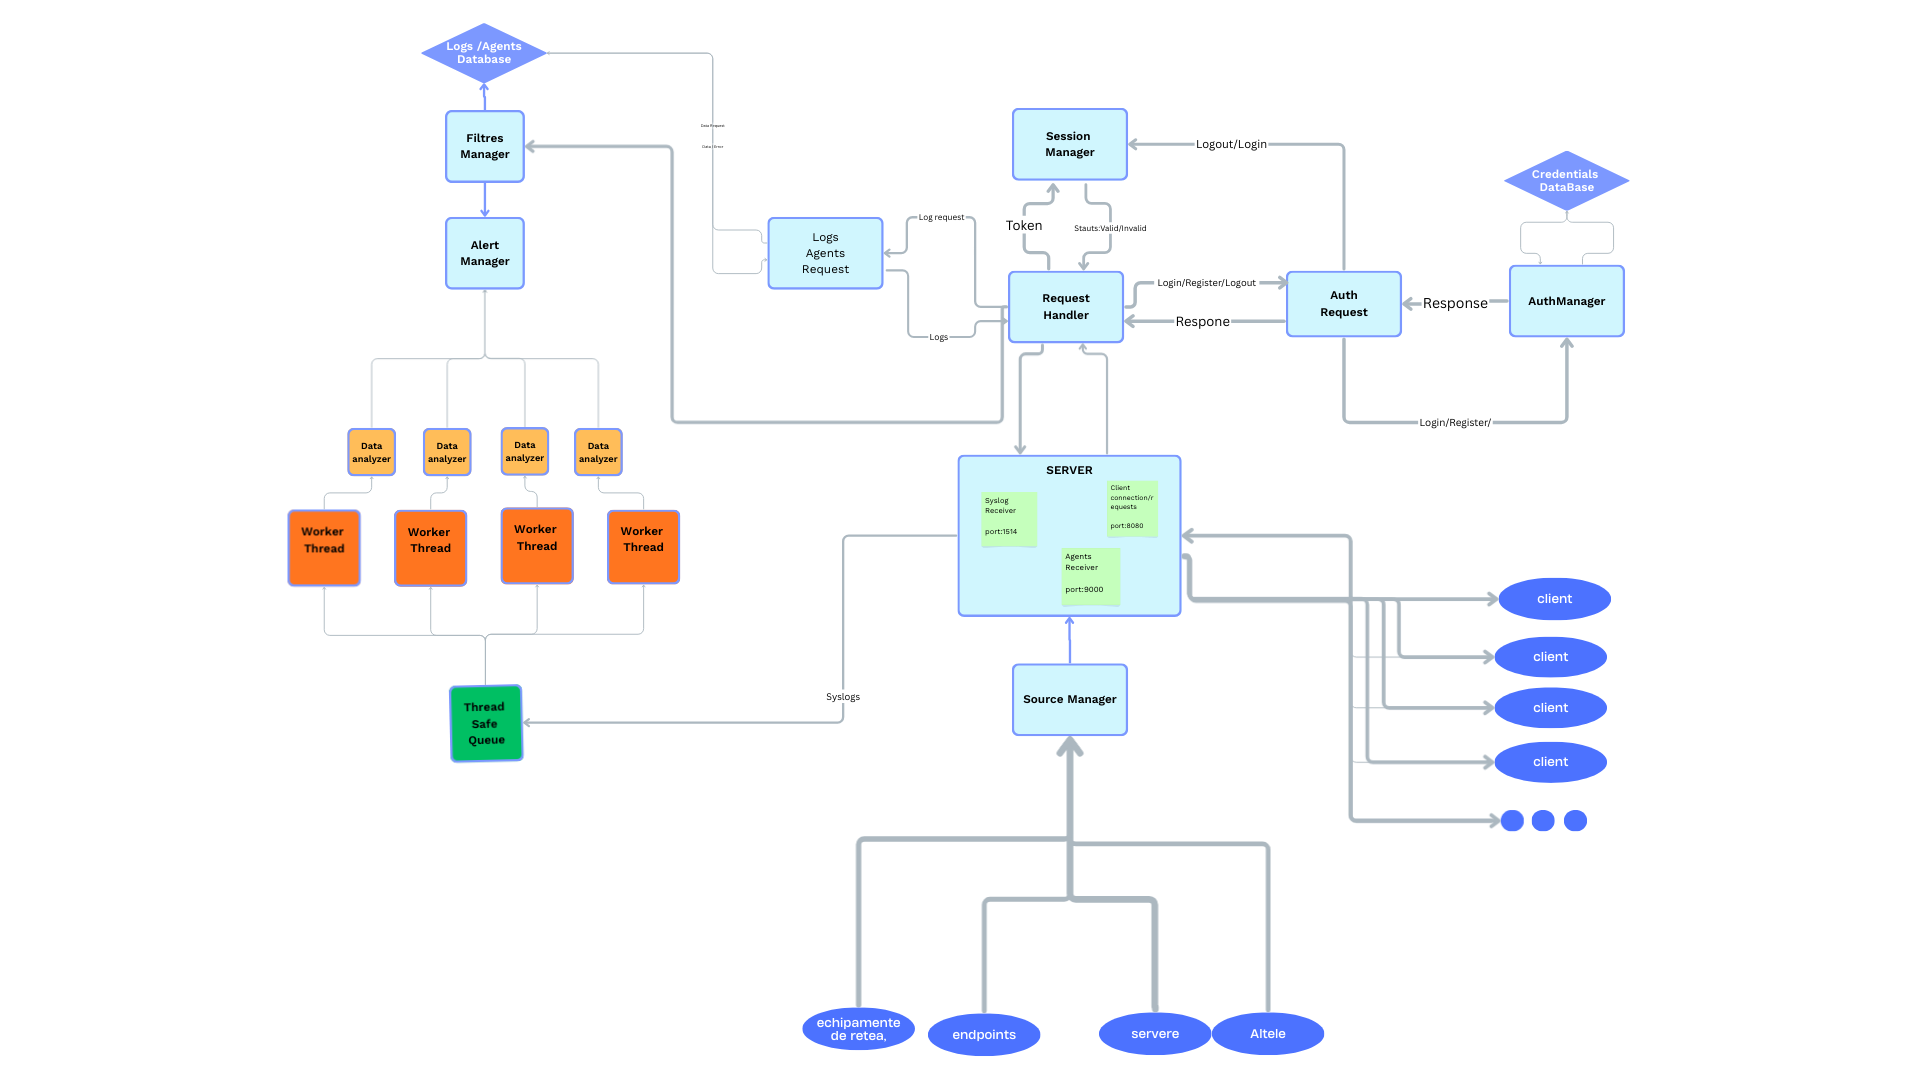
\includegraphics[width=\textwidth]{diagram.png} 
    \caption{Arhitectura completa NetworkDevicesMonitor}
    \label{fig:architecture}
\end{figure}

\subsubsection{1. Server Backend (C++23)}
Inima sistemului, responsabila pentru: 
\begin{itemize}
    \item Receptia si procesarea datelor de pe 3 canale TCP simultane
    \item Management baze de date SQLite3 cu WAL mode pentru concurenta
    \item Autentificare, autorizare si management sesiuni cu token-based auth
    \item Detectare si notificare alerte bazate pe pattern-uri
    \item Filtrare multi-nivel:  source IP, tip mesaj, keyword matching
    \item Procesare paralela cu thread pools
\end{itemize}

\textbf{Componente principale:}
\begin{itemize}
    \item \texttt{LogPipeline} - Orchestrare flux de date
    \item \texttt{SyslogReceiver} - Port 1514, RFC 5424 parsing
    \item \texttt{AgentsReceiver} - Port 9000, JSON metrics
    \item \texttt{ConnectionServer} - Port 8080, Admin API
    \item \texttt{DataProcessor} - Analiza si stocare
    \item \texttt{SourceManager} - Whitelist/Blacklist
    \item \texttt{AlertsManager} - Detectare si management alerte
    \item \texttt{FiltresManager} - Sistem de filtrare avansata
    \item \texttt{DBManager} - Thread-safe database operations
\end{itemize}

\subsubsection{2. Client GUI (Qt6)}
Interfata grafica profesionala cu: 
\begin{itemize}
    \item Sistem de pagini modular cu lifecycle hooks (on\_enter/on\_exit)
    \item Comunicare asincrona (Qt Signals \& Slots)
    \item Vizualizari tabelare
    \item Grafice în timp real cu QtCharts
    \item Popup-uri pentru alerte
\end{itemize}

\textbf{Pagini implementate:}
\begin{enumerate}
    \item \textbf{ConnectPage} - Conectare la server (IP + port)
    \item \textbf{LoginPage} - Autentificare utilizator
    \item \textbf{HomePage} - Dashboard principal cu tiles de navigare
    \item \textbf{DashboardPage} - 4 sub-pagini: 
        \begin{itemize}
            \item Syslog Dashboard (tabele + donut/line charts)
            \item Agents Dashboard (metrici în timp real)
            \item Unknown Syslog Data (trafic neautorizat)
            \item Unknown Agent Data (agenti necunoscuti)
        \end{itemize}
    \item \textbf{SecurityPage} - Management Whitelist/Blacklist cu add/remove
    \item \textbf{AlertsPage} - Vizualizare si rezolvare alerte
    \item \textbf{FiltresPage} - Configurare filtre (type, message, custom alerts)
    \item \textbf{SettingsPage} - Configurari aplicatie
\end{enumerate}

\subsection{Pipeline-ul de Date}

\subsubsection{Port 1514 - Syslog Receiver}
\textbf{Fluxul de procesare:}

\begin{enumerate}
    \item \textbf{Receptie: } Thread dedicat cu \texttt{poll()} monitorizeaza socket-ul
    \item \textbf{Validare IP:} Source Manager verifica whitelist/blacklist
    \item \textbf{Parsare: } Extragere campuri conform RFC 5424:
    \begin{itemize}
        \item PRI (Priority = Facility × 8 + Severity)
        \item Timestamp 
        \item Hostname
        \item Source (proces/serviciu)
        \item Message content
    \end{itemize}
    \item \textbf{Filtrare:} FiltresManager aplica reguli (type, message keywords)
    \item \textbf{Analiza:} AlertsManager detecteaza pattern-uri suspecte
    \item \textbf{Stocare:} Insert în \texttt{logs} (known) sau \texttt{unknown\_log}
\end{enumerate}

\textbf{Exemplu mesaj Syslog procesat:}
\begin{lstlisting}
<13>1 2025-11-27T15:37:44Z server02 sshd 3452 - - 
Accepted password for user_valid from 192.168.2.5
\end{lstlisting}

\textbf{Implementare în cod:}
\begin{lstlisting}
// server/src/log_pipeline/syslog_server/SyslogReceiver.cpp
void SyslogReceiver::start() {
    std::vector<pollfd> fds;
    pollfd server_poll = {server_fd. value(), POLLIN, 0};
    fds.push_back(server_poll);
    
    while(true) {
        poll(fds.data(), fds.size(), -1);
        for (auto& fd : fds) {
            if (!(fd.revents & POLLIN)) continue;
            
            if (fd.fd == server_fd.value()) {
                // Accept new connection
                int client_fd = accept(... );
                std::string ip = get_client_ip(client_fd);
                
                // Security check
                if(source_manager->check_ip_blacklist(ip)) {
                    close(client_fd);
                    continue;
                }
                
                client_ips[client_fd] = ip;
                fds.push_back({client_fd, POLLIN, 0});
            } else {
                // Read data from existing client
                RW_logs(fd.fd);
            }
        }
    }
}
\end{lstlisting}

\subsubsection{Port 9000 - Agent Receiver}
\textbf{Protocol de comunicare:}
\begin{itemize}
    \item Header binar:  4 bytes = lungime payload
    \item Payload JSON cu metrici
\end{itemize}

\begin{lstlisting}[language=Python]
{
  "hostname": "workstation-01",
  "ip_address": "192.168.1.10",
  "os_info": "Linux",
  "cpu_load": 45.2,
  "ram_usage": 68.5,
  "disk_usage": 72.1,
  "status_message": "OK",
  "active_user": "admin"
}
\end{lstlisting}


\subsubsection{Port 8080 - Admin API}
\textbf{Protocol custom JUNK (Just Useful Notation Kinda):}

Format:  \texttt{key:\{value\};key2:\{value2\};}

\textbf{Exemplu cerere login:}
\begin{lstlisting}
type:{login};username:{admin};password:{pass123};
\end{lstlisting}

\textbf{Exemplu raspuns:}
\begin{lstlisting}
succes:{true};type:{login};content:{token_abc123xyz};
\end{lstlisting}

\textbf{Implementare JUNK Parser:}
\begin{lstlisting}
// server/src/utils/JUNK. cpp
std::expected<JUNK, std::string> JUNK::deserialize(std::string data) {
    JUNK new_data;
    int left_count = 0, format_count = 0, poz = 0;
    std::string key_val[2];
    
    for(auto ch : data) {
        if (ch == '\n' || ch == '\r') continue;
        
        if(ch == ': ' && left_count == 0) {
            poz = 1;
            format_count++;
            continue;
        }
        if(ch == '{') {
            left_count++;
            if (left_count == 1) continue;
        }
        if(ch == '}') {
            left_count--;
            if (left_count == 0) continue;
        }
        if(ch == ';' && left_count == 0) {
            new_data.add(key_val[0], key_val[1]);
            poz = 0;
            key_val[0]. clear();
            key_val[1].clear();
            continue;
        }
        key_val[poz].push_back(ch);
    }
    
    if(format_count == 0 || left_count != 0 || new_data.empty())
        return std::unexpected("Invalid JUNK format");
    return new_data;
}
\end{lstlisting}

\section{Implementare Tehnica Detaliata}

\subsection{Server:  Concurenta si Thread Safety}

\subsubsection{Thread-Safe Queue Implementation}
Pattern Producer-Consumer pentru decuplarea I/O de procesare:

\begin{lstlisting}
// server/src/utils/ThreadSafeQueue.hpp
template<class T>
class ThreadSafeQueue {
    std::queue<T> queue;
    std::mutex _mutex;
    
public:
    void push(T value) {
        std::lock_guard<std::mutex> lock(_mutex);
        this->queue.push(value);
    }
    
    std:: expected<T, std::string> pop() {
        std::lock_guard<std::mutex> lock(_mutex);
        if(queue.empty()) 
            return std::unexpected("Empty queue");
        auto value = queue.front();
        queue.pop();
        return value;
    }
};

// Event structure
enum EventType { SYSLOG, AGENT_METRIC };
struct LogEvent {
    EventType type;
    std::string source_ip;
    std::string payload;
};
\end{lstlisting}

\subsubsection{Database Manager (SQLite3 WAL Mode)}
\textbf{Caracteristici cheie:}
\begin{itemize}
    \item \texttt{shared\_mutex} pentru Read-Write locking concurrent
    \item Prepared statements pentru securitate anti-SQL injection
    \item WAL (Write-Ahead Logging) pentru citiri simultane

\end{itemize}

\textbf{Tabele principale:}
\begin{enumerate}
    \item \texttt{logs} - Syslog-uri de la surse cunoscute (whitelist)
    \item \texttt{unknown\_log} - Trafic de la surse necunoscute
    \item \texttt{agents\_metrics} - Date de la agenti de monitorizare
    \item \texttt{users} - Credentiale administratori (token-based auth)
    \item \texttt{whitelist} - Surse validate (IP + hostname)
    \item \texttt{blacklist} - Surse blocate
    \item \texttt{alerts} - Evenimente critice detectate
    \item \texttt{filtres\_type} - Filtre pe tip de log
    \item \texttt{filtres\_message} - Filtre pe keyword în mesaj
    \item \texttt{filtres\_alerts} - Alerte personalizate
\end{enumerate}


\subsubsection{Source Manager - Sistem de Securitate}
\textbf{Operatiuni principale:}

\begin{lstlisting}
// server/src/log_pipeline/source_managers/SourceManager.hpp
class SourceManager {
    std::shared_mutex _mutex;
    std::unordered_map<std::string, std::string> 
        whitelist_source;  // IP -> Hostname
    std::unordered_set<std::string> blacklist_source;
    std::shared_ptr<DBManager> db;
    
public:
    std::optional<std::string> check_ip_whitelist(std::string ip) {
        std::shared_lock lock(_mutex);
        if(whitelist_source.contains(ip))
            return whitelist_source[ip];
        return std::nullopt;
    }
    
    bool check_ip_blacklist(std::string ip) {
        std::shared_lock lock(_mutex);
        return blacklist_source.contains(ip);
    }
    
    void add_to_whitelist(std::string ip, std::string hostname) {
        std::unique_lock lock(_mutex);
        whitelist_source[ip] = hostname;
        // Persist to DB
        db->query("INSERT INTO whitelist VALUES (?, ?)", {ip, hostname});
    }
    
    void add_to_blacklist(std:: string ip) {
        std::unique_lock lock(_mutex);
        blacklist_source.insert(ip);
        db->query("INSERT INTO blacklist VALUES (?)", {ip});
    }
};
\end{lstlisting}

\subsection{Sistem de Filtrare Avansata}

\subsubsection{FiltresManager - Filtrare Multi-Nivel}
Sistemul implementeaza 3 tipuri de filtre: 

\textbf{1. Filtre pe Tip (Type Filters):}
\begin{itemize}
    \item Filtreaza log-uri dupa tipul evenimentului
    \item Matching exact pe campul \texttt{severity}
    \item Utilizare:  exclude log-uri non-critice
\end{itemize}

\textbf{2. Filtre pe Mesaj (Message Filters):}
\begin{itemize}
    \item Keyword matching în corpul mesajului
    \item Case-insensitive search
    \item Utilizare:  cauta pattern-uri specifice (error, failed, denied)
\end{itemize}

\textbf{3. Alerte Personalizate (Custom Alerts):}
\begin{itemize}
    \item Declansare alerte pe keyword-uri critice
    \item Notificare instant catre clienti conectati
    \item Severitate configurabila
\end{itemize}




\subsection{Sistem de Alertare}

\subsubsection{AlertsManager (Server)}
\textbf{Detectare pattern-uri suspecte:}
\begin{itemize}
    \item Tentative repetate de login (sper ca am terminat asta)
    \item Trafic de pe IP-uri din blacklist
    \item Consum CPU/RAM peste threshold-uri (>90\% pentru >30 sec)
    \item Keyword matching din filtre custom
\end{itemize}


\subsubsection{AlertsPage si AlertPopup (Client)}

\textbf{AlertsPage - Management centralizat:}
\begin{itemize}
    \item Tabel cu toate alertele (ID, Type, Severity, Source, Message, Timestamp)
    \item Buton "Resolve" pentru marcarea alertelor ca rezolvate
    \item Auto-refresh la interval de 2 secunde
\end{itemize}

\textbf{AlertPopup - Notificari non-intruzive:}
\begin{lstlisting}
// client/src/frontend/widgets/AlertPopup.cpp
class AlertPopup : public QWidget {
public:
    void showMessage(QString title, QString message, bool isCritical) {
        titleLabel->setText(title);
        messageLabel->setText(message);
        
        if(isCritical) {
            setStyleSheet(R"(
                QWidget {
                    background-color: #2C1B1B;
                    border-left: 5px solid #FF5555;
                }
            )");
        } else {
            setStyleSheet(R"(
                QWidget {
                    background-color: #2C2416;
                    border-left:  5px solid #F1C40F;
                }
            )");
        }
        
        // Show in bottom-right corner
        QScreen *screen = QApplication::primaryScreen();
        QRect screenGeometry = screen->geometry();
        int x = screenGeometry.width() - this->width() - 20;
        int y = screenGeometry.height() - this->height() - 20;
        this->move(x, y);
        
        this->show();
        
        // Auto-hide after 10 seconds
        QTimer::singleShot(10000, this, &AlertPopup::hide);
    }
};
\end{lstlisting}

\textbf{Integrare cu DataRequester:}
\begin{lstlisting}
// client/src/frontend/app. cpp
connect(data_requester.get(), &DataRequester::UpdateAlertsPopup, 
    this, [this](QString data) {
        auto junk = JUNK::deserialize(data.toStdString());
        if(!junk.has_value() || junk.value()["succes"].value() == "false")
            return;
            
        auto alerts_str = junk.value()["content"].value();
        auto alerts = parse_alerts(alerts_str);
        
        for(const auto& alert : alerts) {
            if(alert.id > last_alert_id) {
                bool isCritical = (alert.severity == "high" || 
                                  alert.severity == "critical");
                alert_popup->showMessage(
                    QString:: fromStdString(alert.type),
                    QString::fromStdString(alert.message),
                    isCritical
                );
                last_alert_id = alert.id;
            }
        }
    });
\end{lstlisting}

\subsection{Client:  Interfata Grafica Asincrona}

\subsubsection{Page Management System}
Arhitectura modulara pentru navigare cu lifecycle management:

\begin{lstlisting}
// client/src/frontend/page_system/PageManager.h
class PageManager {
    std::shared_ptr<QStackedWidget> stack;
    std::vector<std::shared_ptr<Page>> pages;
    std::shared_ptr<Page> current_page;
    
public:
    void change_page(int index) {
        if(current_page)
            current_page->on_exit();  // Cleanup
        
        stack->setCurrentIndex(index);
        current_page = pages->at(index);
        current_page->on_enter();  // Initialize
    }
    
    void add_page(QWidget* page_widget) {
        stack->addWidget(page_widget);
    }
};

// Abstract base class
class Page {
protected:
    QWidget* page;
    std::shared_ptr<DataRequester> data_requester;
    std::shared_ptr<PageManager> page_manager;
    std::shared_ptr<QMainWindow> window;
    
public:
    virtual void on_enter() = 0;  // Called when page becomes active
    virtual void on_exit() = 0;   // Called when leaving page
    QWidget* get_page() { return page; }
};
\end{lstlisting}


\subsubsection{Comunicare Asincrona cu Signals}

\begin{lstlisting}
// client/src/server_request/DataRequester.h
class DataRequester :  public QObject {
    Q_OBJECT
    
signals:
    void LoginData(QString data);
    void LogsData(QString data);
    void UpdateAlertsDashboard(QString response);
    void UpdateWhitelist(QString response);
    void UpdateBlacklist(QString response);
    void UpdateAlertsPopup(QString response);
    void UpdateSyslogDashboard(QString response);
    void UpdateAgentsDashboard(QString response);
    void UpdateUnknownSyslog(QString response);
    void UpdateUnknownAgent(QString response);
    void UpdateFiltres(QString response);
    void lost_connection();
    
public slots:
    void start_receiving() {
        while(connected) {
            auto packet = receive();
            if(! packet.has_value()) {
                emit lost_connection();
                break;
            }
            
            auto junk = JUNK::deserialize(packet.value());
            if(! junk.has_value()) continue;
            
            std::string type = junk.value()["type"].value_or("");
            
            if(type == "login")
                emit LoginData(QString::fromStdString(packet.value()));
            else if(type == "logs")
                emit LogsData(QString::fromStdString(packet.value()));
            else if(type == "alerts")
                emit UpdateAlertsDashboard(QString::fromStdString(packet.value()));
            // ... etc pentru toate tipurile
        }
    }
};
\end{lstlisting}

\textbf{Conectare în UI:}
\begin{lstlisting}
// client/src/frontend/app.cpp
connect(data_requester.get(), &DataRequester::LogsData, 
    this, [this](QString data) {
        auto junk = JUNK:: deserialize(data.toStdString());
        if(!junk.has_value()) return;
        
        auto logs_str = junk.value()["content"].value();
        auto logs = BetterString::split(logs_str, ": ;:");
        
        // Update table
        syslog_dashboard->update_table(logs);
        
        // Update charts
        syslog_dashboard->update_charts(logs);
    });
\end{lstlisting}

\subsubsection{Security Page - Whitelist/Blacklist Management}

\textbf{Functionalitati: }
\begin{itemize}
    \item 2 tab-uri: Whitelist si Blacklist
    \item Tabel cu IP si Hostname (whitelist) sau doar IP (blacklist)
    \item Buton "Add" deschide popup modal
    \item Delete la click pe rand în tabel
    \item Sincronizare instant cu server
    \item Conflict detection (IP deja în cealalta lista)
\end{itemize}

\section{Protocol de Comunicare}

\subsection{Structura Pachetului (Admin API)}

\begin{table}[H]
\centering
\begin{tabular}{|l|l|l|}
\hline
\textbf{Bytes} & \textbf{Tip} & \textbf{Descriere} \\ \hline
0-3 & int & Lungime payload \\ \hline
4-N & ASCII Text & Date în format JUNK \\ \hline
\end{tabular}
\caption{Format pachet TCP pe port 8080}
\end{table}

\subsection{Comenzi Disponibile}

\begin{table}[H]
\centering
\small
\begin{tabular}{|l|p{10cm}|}
\hline
\textbf{Comanda} & \textbf{Format cerere} \\ \hline
Login & \texttt{type:\{login\};username:\{.. .\};password:\{...\};} \\ \hline
Register & \texttt{type:\{register\};username:\{...\};password:\{...\};} \\ \hline
Get Logs & \texttt{type:\{logs\};last\_id:\{123\};token:\{...\};} \\ \hline
Get Agents & \texttt{type:\{agents\};last\_id:\{0\};token:\{...\};} \\ \hline
Add Whitelist & \texttt{type:\{add\_whitelist\};ip:\{.. .\};hostname:\{...\};token:\{...\};} \\ \hline
Add Blacklist & \texttt{type:\{add\_blacklist\};ip:\{...\};token:\{...\};} \\ \hline
Remove Whitelist & \texttt{type:\{remove\_whitelist\};ip:\{...\};token:\{.. .\};} \\ \hline
Remove Blacklist & \texttt{type:\{remove\_blacklist\};ip:\{...\};token:\{...\};} \\ \hline
Get Alerts & \texttt{type:\{update\_alerts\};last\_id:\{0\};token:\{...\};} \\ \hline
Resolve Alert & \texttt{type:\{remove\_alert\};alert\_id:\{123\};token:\{...\};} \\ \hline
Add Type Filter & \texttt{type:\{add\_type\_filter\};keyword:\{SSH\};token:\{...\};} \\ \hline
Add Msg Filter & \texttt{type:\{add\_msg\_filter\};keyword:\{error\};token:\{...\};} \\ \hline
Add Custom Alert & \texttt{type:\{add\_custom\_alert\};keyword:\{critical\};token:\{...\};} \\ \hline
Get Filtres & \texttt{type:\{get\_filtres\};token:\{...\};} \\ \hline
Unknown Syslog & \texttt{type:\{unknown\_syslog\};last\_id:\{0\};token:\{...\};} \\ \hline
Unknown Agents & \texttt{type:\{unknown\_agents\};last\_id:\{0\};token:\{...\};} \\ \hline
\end{tabular}
\caption{API endpoints complete}
\end{table}

\subsection{Exemple de Raspunsuri}

\textbf{Raspuns succes login:}
\begin{lstlisting}
succes:{true};type:{login};content:{eyJhbGciOiJIUzI1NiIsInR5cCI6IkpXVCJ9};
\end{lstlisting}

\textbf{Raspuns logs:}
\begin{lstlisting}
succes:{true};type:{logs};content:{
    1[]2025-11-27 15:30:00[]4[]server01[]sshd[]Login successful: ;: 
    2[]2025-11-27 15:31:00[]3[]router01[]firewall[]Blocked connection:;:
};
\end{lstlisting}

\textbf{Raspuns eroare:}
\begin{lstlisting}
succes:{false};type:{error};content:{Invalid token};
\end{lstlisting}

\subsection{Validare cu Wireshark}

\begin{figure}[H]
    \centering
    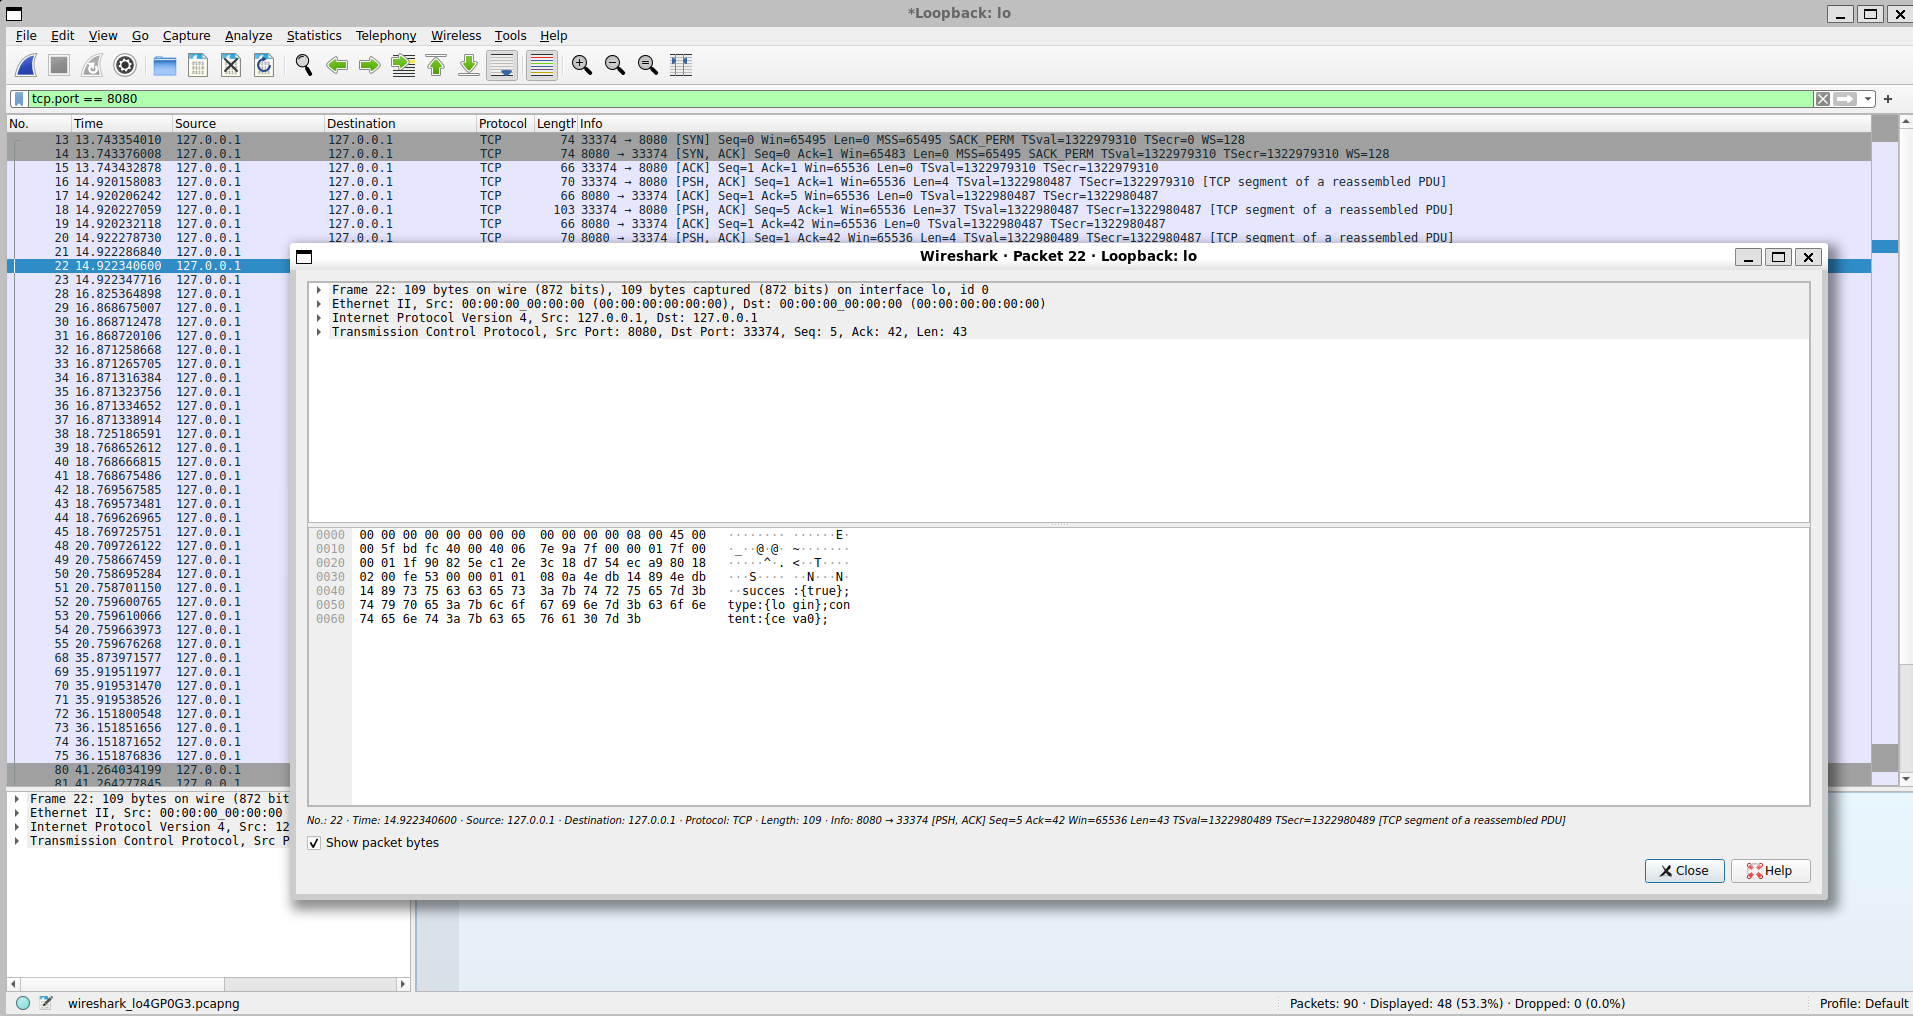
\includegraphics[width=\textwidth]{exemplu1WIRESHARK.png} 
    \caption{Captura Wireshark - Analiza pachetelor JUNK}
    \label{fig:wireshark}
\end{figure}


\section{Scenarii de Utilizare}

\subsection{Scenarii de Succes}

\subsubsection{Scenariu 1: Monitorizare Agent în Timp Real}
\textbf{Context:} Un server de baze de date PostgreSQL trimite metrici la interval de 5 secunde. 

\textbf{Flow:}
\begin{enumerate}
    \item Agent Python colecteaza date cu \texttt{psutil}: 
    \begin{lstlisting}[language=Python]
cpu_load = psutil.cpu_percent(interval=1)
ram_usage = psutil.virtual_memory().percent
disk_usage = psutil.disk_usage('/').percent
    \end{lstlisting}
    \item Pachet JSON trimis pe port 9000 cu header binar
    \item Server primeste, valideaza IP în whitelist via SourceManager
    \item DataProcessor extrage metrici, insert în \texttt{agents\_metrics}
    \item Client primeste signal \texttt{AgentDataUpdated}
    \item Dashboard actualizeaza grafic CPU/RAM automat fara refresh
\end{enumerate}

\textbf{Rezultat:} Administrator vizualizeaza în sub 3 secunda cresterea CPU la 92\%, investigare preventiva înainte de crash.

\subsubsection{Scenariu 2: Onboarding Echipament Nou}

\textbf{Flow:}
\begin{enumerate}
    \item Admin acceseaza SecurityPage → Whitelist tab
    \item Click "Add Source", completeaza în popup:  
    \begin{itemize}
        \item IP: 192.168.10.50
        \item Hostname: switch-floor2
    \end{itemize}
    \item Click "Add" → cerere JUNK trimisa la server: 
    \begin{lstlisting}
type:{add_whitelist};ip:{192.168.10.50};hostname:{switch-floor2};
    \end{lstlisting}
    \item SourceManager insereaza în DB + hash map in-memory
    \item Switch-ul configureaza syslog destination catre server: 1514
    \item Primul syslog primit, IP verificat în whitelist → ACCEPTED
    \item Procesat imediat, apare în Syslog Dashboard cu label "switch-floor2"
    \item Donut chart actualizat cu noi date
\end{enumerate}

\textbf{Rezultat:} Zero downtime, instant visibility pentru noul device.

\subsubsection{Scenariu 3: Configurare Filtre Custom}
\textbf{Context:} Admin vrea sa ignore log-uri verbose de la servere web (HTTP 200 OK).

\textbf{Flow:}
\begin{enumerate}
    \item Acceseaza FiltresPage → Message Filters tab
    \item Click "Add Message Filter"
    \item Introduce keyword: "HTTP 200"
    \item Server adauga în \texttt{filtres\_message} table
    \item FiltresManager încarca în memory cache
    \item Log-uri urmatoare cu "HTTP 200" sunt filtrate automat
    \item Dashboard ramane clean cu doar evenimente relevante
\end{enumerate}

\textbf{Rezultat:} Reducere zgomotul în dashboard, focus pe evenimente critice.

\subsubsection{Scenariu 4: Alerta Personalizata pe Keyword}
\textbf{Context:} Admin vrea notificare instant la orice mesaj continand "OutOfMemory".

\textbf{Flow:}
\begin{enumerate}
    \item FiltresPage → Custom Alerts tab → "Add Custom Alert"
    \item Introduce keyword: "OutOfMemory"
    \item Server adauga în \texttt{filtres\_alerts}
    \item Un serviciu Java crasheaza cu "java.lang.OutOfMemoryError"
    \item Log syslog primit, DataProcessor match keyword
    \item AlertsManager creeaza alerta CRITICAL
    \item Popup instant la client: "OutOfMemory error detected on app-server-03"
    \item Admin verifica AlertsPage, vede stack trace complet
\end{enumerate}

\textbf{Rezultat:} Detectie proactiva, restart serviciu înainte de afectare utilizatori.

\subsection{Scenarii de Esec si Recuperare}

\subsubsection{Scenariu 5: Trafic Malitios Blocat}
\textbf{Context:} Botnet încearca flood de date false pe port 1514.

\textbf{Flow:}
\begin{enumerate}
    \item 1000 de pachete/sec de pe IP 198.51.100.10 (în blacklist)
    \item SyslogReceiver detecteaza conexiune în \texttt{accept()}
    \item SourceManager verifica:  \texttt{check\_ip\_blacklist()} → \texttt{true}
    \item Socket închis imediat cu \texttt{close(client\_fd)}, zero processing
    \item Log în \texttt{security\_events}:  "Blocked blacklist IP 198.51.100.10"
    \item Statistici actualizate:  "X blocked attempts today"
\end{enumerate}

\textbf{Rezultat:} Zero impact pe performanta, CPU usage normal (<5\%).

\subsubsection{Scenariu 6: Pachet Corupt Primit}
\textbf{Context:} Eroare de retea corupe header-ul unui pachet JUNK.

\textbf{Flow:}
\begin{enumerate}
    \item Client trimite pachet cu lungime incorecta în header (0xFFFFFFFF)
    \item Server citeste 4 bytes:  \texttt{length = 4294967295} (invalid)
    \item Buffer allocation failsafe: maxim 64KB hardcoded
    \item Alloc doar 64KB, citire partiala
    \item \texttt{JUNK:: deserialize()} returneaza \texttt{std::unexpected("Invalid format")}
    \item RequestHandler logheaza eroare, trimite:  
    \begin{lstlisting}
succes:{false};type:{error};content:{Invalid JUNK format};
    \end{lstlisting}
    \item Client afiseaza QMessageBox:  "Request failed, please retry"
\end{enumerate}

\textbf{Rezultat:} Server nu crasheaza, conexiune mentinuta, utilizator poate re-trimite.

\subsubsection{Scenariu 7: Token Expirat}
\textbf{Context:} Admin lasa aplicatia deschisa 24h, sesiune expirata pe server.

\textbf{Flow:}
\begin{enumerate}
    \item Client încearca sa ceara logs cu token vechi
    \item SessionManager verifica:  token nu mai exista în hash map (cleared dupa 12h)
    \item Raspuns: \texttt{succes:\{false\};type:\{error\};content:\{Session expired\};}
\end{enumerate}

\textbf{Rezultat: } Security enforcement, experienta user fluida.

\section{Concluzii}

Acest proiect a fost, înainte de toate, o experienta de învatare foarte utila. Daca la început totul era doar o schita, acum am un server functional (cu Syslog si Agenti) si un client care chiar comunica între ei.

\subsection*{Ce am învatat pe parcurs}
Nu a fost doar despre scris cod, ci despre a întelege cum se leaga lucrurile în prezent:
\begin{itemize}
    \item \textbf{C++23:} Am profitat de ocazie sa explorez noutatile din noul standard pentru a scrie codul mai modern.
    \item \textbf{Concurenta:} Am învatat sa gestionez mai bine firele de executie.
    \item \textbf{Arhitectura:} Am pus mare pret pe modularitate. Faptul ca am împartit totul pe clase si module m-a ajutat enorm sa nu ma pierd în detalii pe masura ce proiectul crestea.
\end{itemize}

\subsection*{O privire realista}
Sunt constient ca proiectul nu este perfect si ca, daca as mai avea timp, ar mai fi destule „colturi de slefuit” sau functionalitati de optimizat. Totusi, pentru stadiul actual, consider ca a iesit un proiect bun, stabil si, cel mai important, usor de înteles datorita structurii sale ordonate. 

A fost o provocare care mi-a aratat exact unde mai am de lucrat, dar si cat de mult am progresat.
\begin{thebibliography}{8}

\bibitem{curs_retele}
Facultatea de Informatica Iasi: Retele de Calculatoare - Resurse Curs si Laborator.\url{https://edu.info.uaic.ro/computer-networks/cursullaboratorul. php}

\bibitem{geeks_thread}
GeeksforGeeks: Multithreading in C++.  \url{https://www.geeksforgeeks.org/cpp/multithreading-in-cpp/}

\bibitem{cpp_expected}
C++ Reference: std::expected (Error handling).  \url{https://en.cppreference.com/w/cpp/utility/expected. html}

\bibitem{splunk_syslog}
Splunk: What is Syslog? A Complete Guide to Syslog Monitoring. \url{https://www. splunk.com/en_us/blog/learn/syslog. html} 
\bibitem{QT - C++}
Qt Documentation \url{https://doc.qt. io/} 

\bibitem{Nlohmann Json}
Json Documentation \url{https://json.nlohmann.me/} 

\bibitem{Sqlite3}
Sqlite \url{https://sqlite.org/cli.html} 


\end{thebibliography}
\end{document}
